\chapter{Detector description}

%versions of the detector
\section{History}

``The desktop muon detector was initially built as a Muon Tagging Optical Modules (MTOMs) for PINGU, the proposed low energy upgrade for IceCube experiment'' \cite{CosmicWatch}. Since the first iteration CosmicWatch has had multiple versions, always aiming to reduce size and costs, simplify its construction and provide better documentation for new CosmicWatch users. An indepth review of the detector evolution can be found in \cite{CosmicWatch} under ``About the project/Project evolution''.

The previous versions of CosmicWatch used an Aduino Nano to process the signal comming from the photomultiplier\footnote{see chapter \ref{chap:Electronics} for an indepth description of the inner workings of the detector electronics}, which has only one core. This is a disadvantage when there is a high event rate, due to the fact that one can not sample data while saving previous events.

Up until now only plastic scintillator had been used, due to how affordable and maleable it can be. Sadly, the poor resolution of this kind of scintillator makes it useless for spectroscopy. in addition to this plastics scintillators like BC-404 have a decay time of  

\section{Plastic vs. LYSO}

\section{Power Consumption}

\section{KiCad}

\section{Accessories}

\section{3D printed case}

In order to hold the crystal in place on the SiPM PCB, it was necessary to design a 3D printed case -see Fig. \ref{fig:3d_case_desing} for an image of the 3D desing on inventor. With this we made sure that the crystal would not move with respect to the SiPM, preventing scratches and providing a more stable optical coupling with the photomultiplier.

\begin{figure}[H]
    \centering
    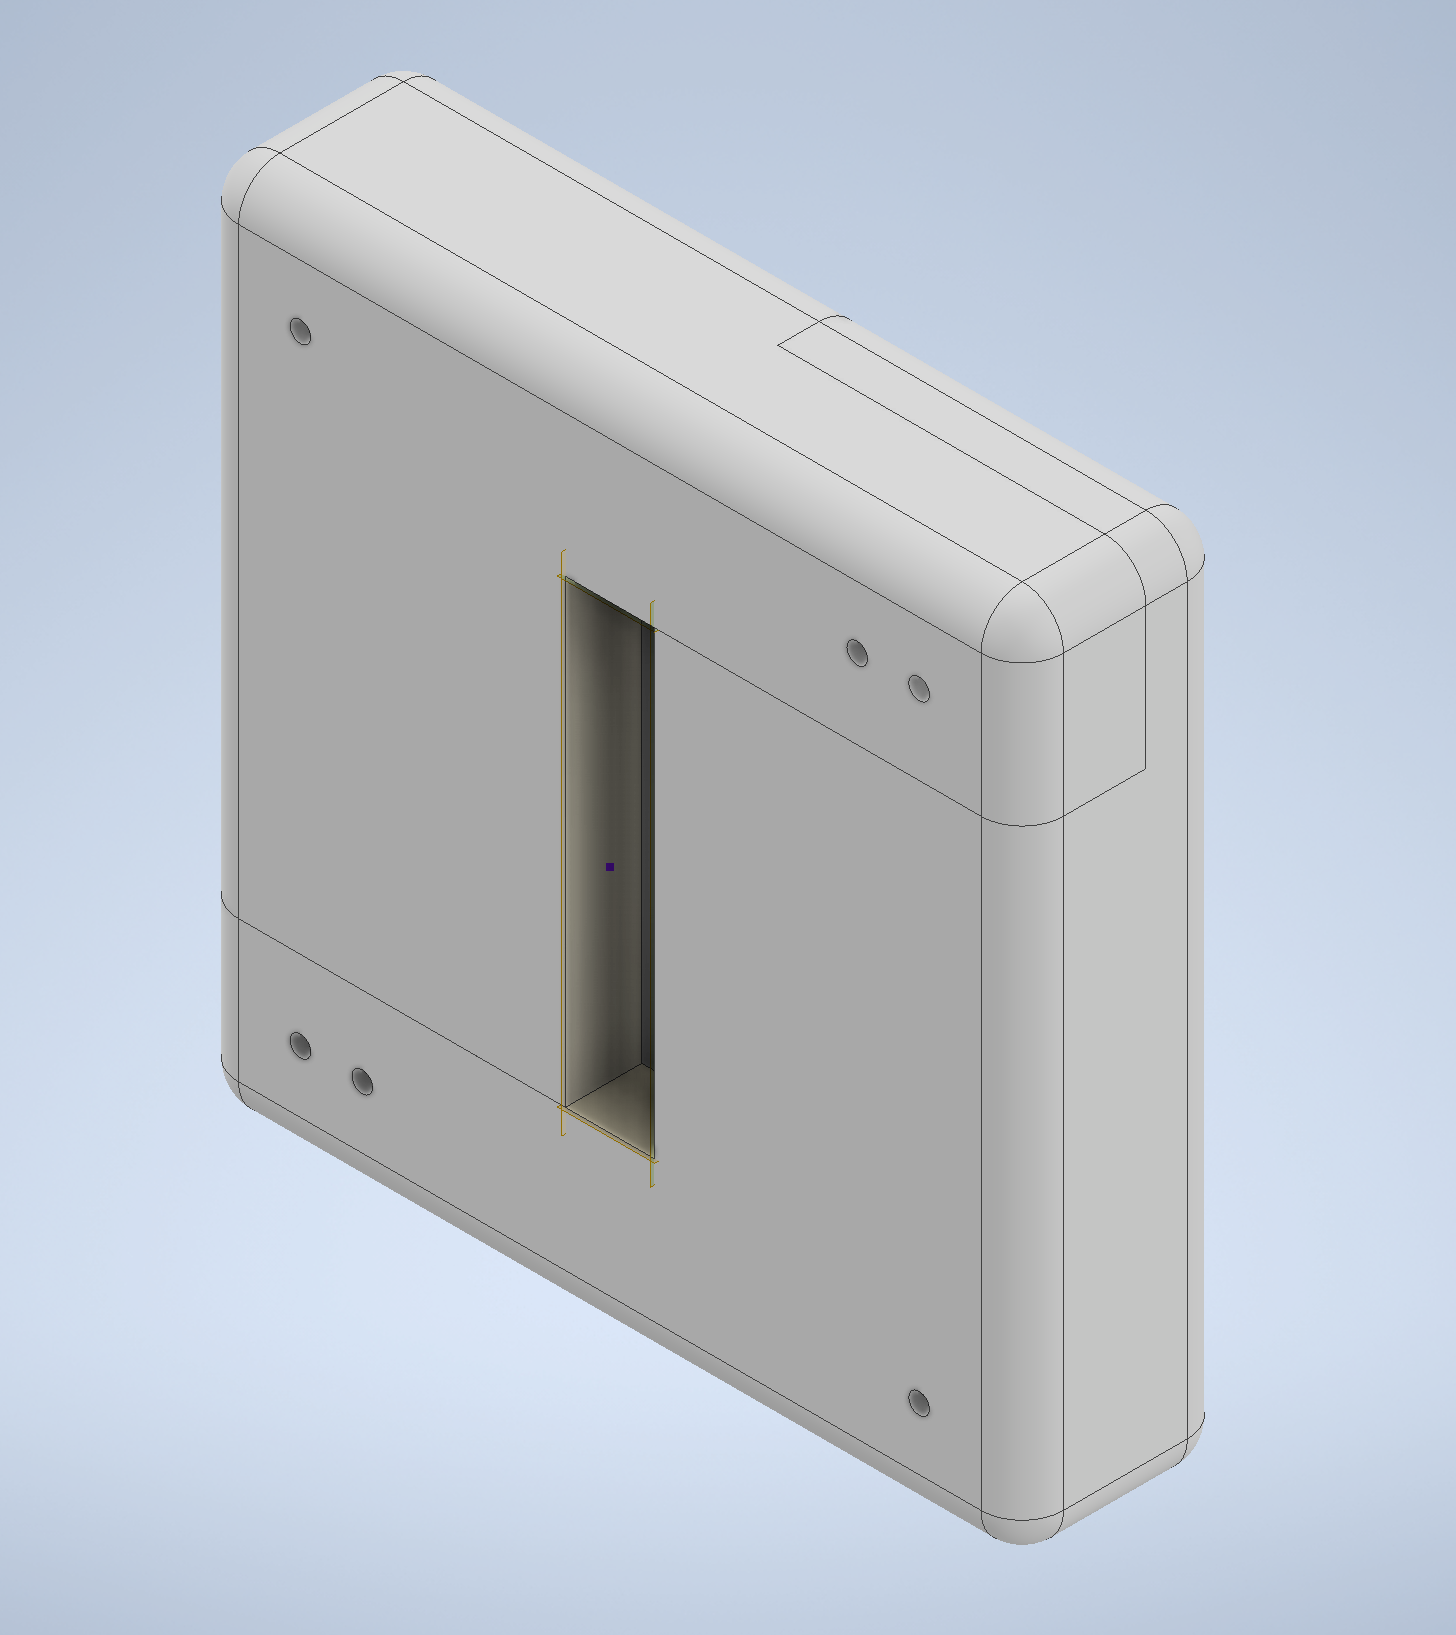
\includegraphics[width=0.6\textwidth]{Detector_description/3d_case_inventor.png}
    \caption{3D model of the LYSO case made on inventor, the .cad files can be found on the repository \href{https://github.com/anvargasl/CosmicWatch-gamma-spectroscopy-PCB}{CosmicWatch-gamma-spectroscopy-PCB}.}
    \label{fig:3d_case_desing}
\end{figure}

The design keeps in mind that the crystal has to be wrapped in teflon tape to increase reflectivity, which is why it comes in two pieces that come together around the crystal, lowering the risk of tears. Once the crystal is placed in the case it can be kept together by means of electrical tape.

Before using teflon tape, the crystal was wrapped in tin foil, which made tears common (Fig. \ref{fig:tin_foil_tear}) and greatly impacted the quality of the spectra that could be obtained with the detector. 

\begin{figure}[H]
    \centering
    \begin{subfigure}[t]{0.45\textwidth}
      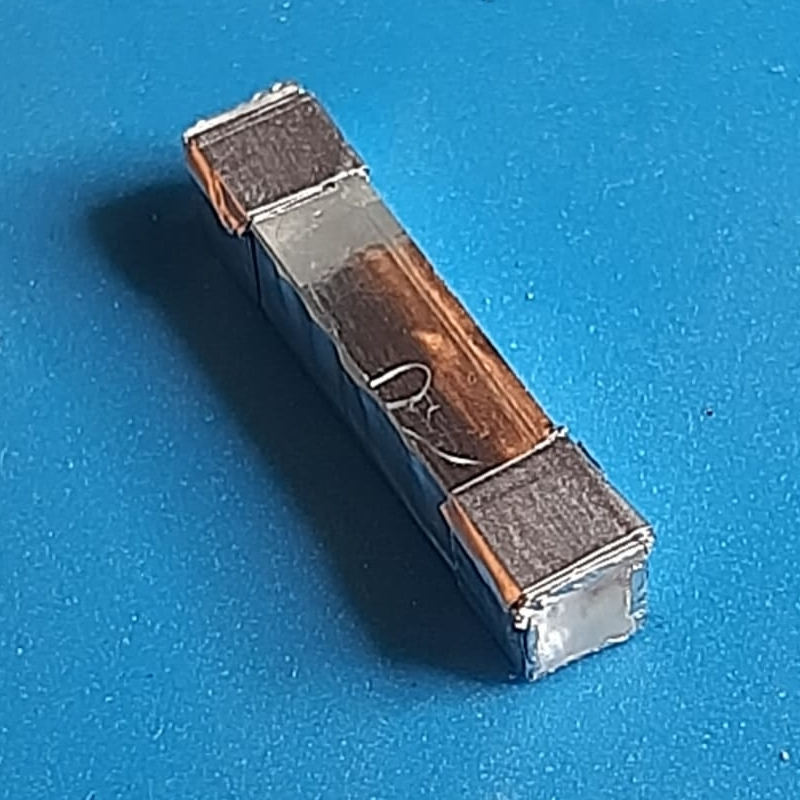
\includegraphics[width=\textwidth]{Detector_description/LYSO-wrapped.jpeg}
    \end{subfigure}
    \begin{subfigure}[t]{0.45\textwidth}
      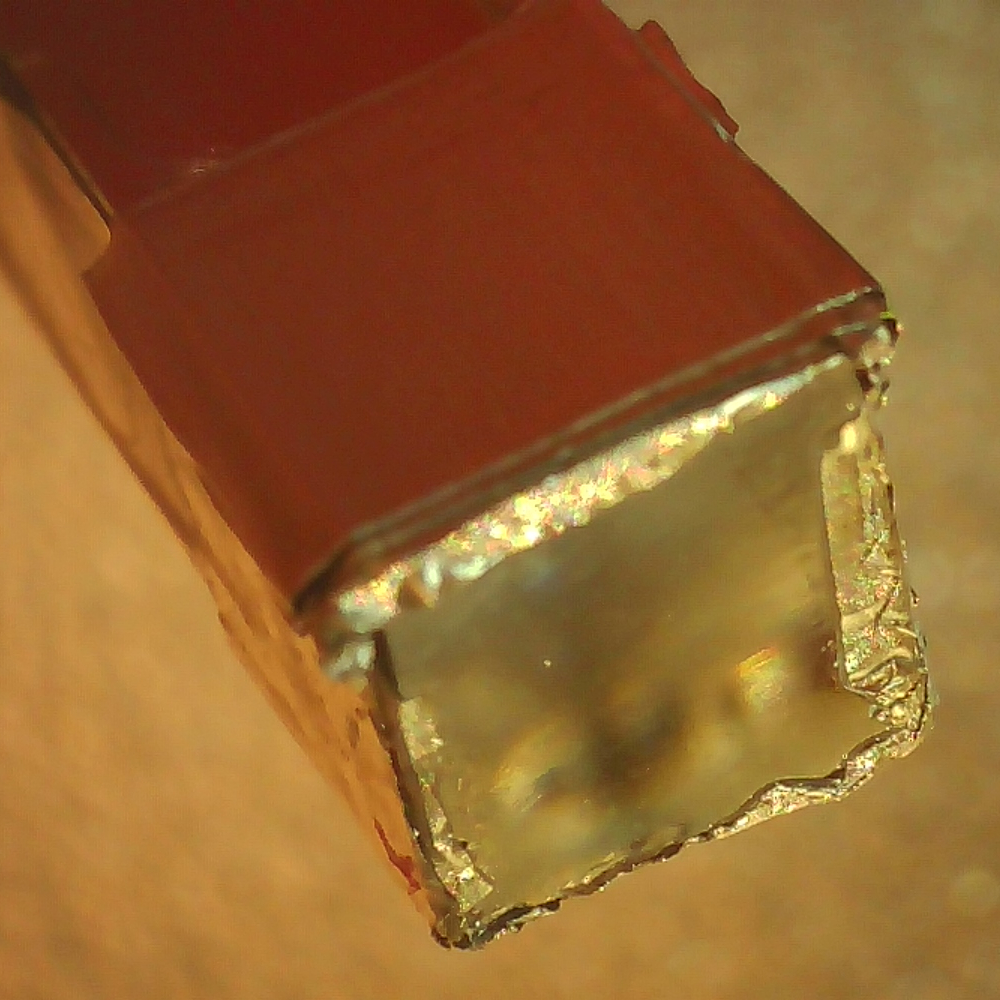
\includegraphics[width=\textwidth]{Detector_description/tin_foil_tear.jpg}
    \end{subfigure}
    \caption{\label{fig:tin_foil_tear}Tin foil tear.}
\end{figure}

Teflon tape seems to solve the tearing problem. However, with the intention to reduce the risk of tearing the teflon, multiple iterations of the case were desined (Fig. \ref{fig:3d_previous_desings})

\begin{figure}[H]
    \centering
    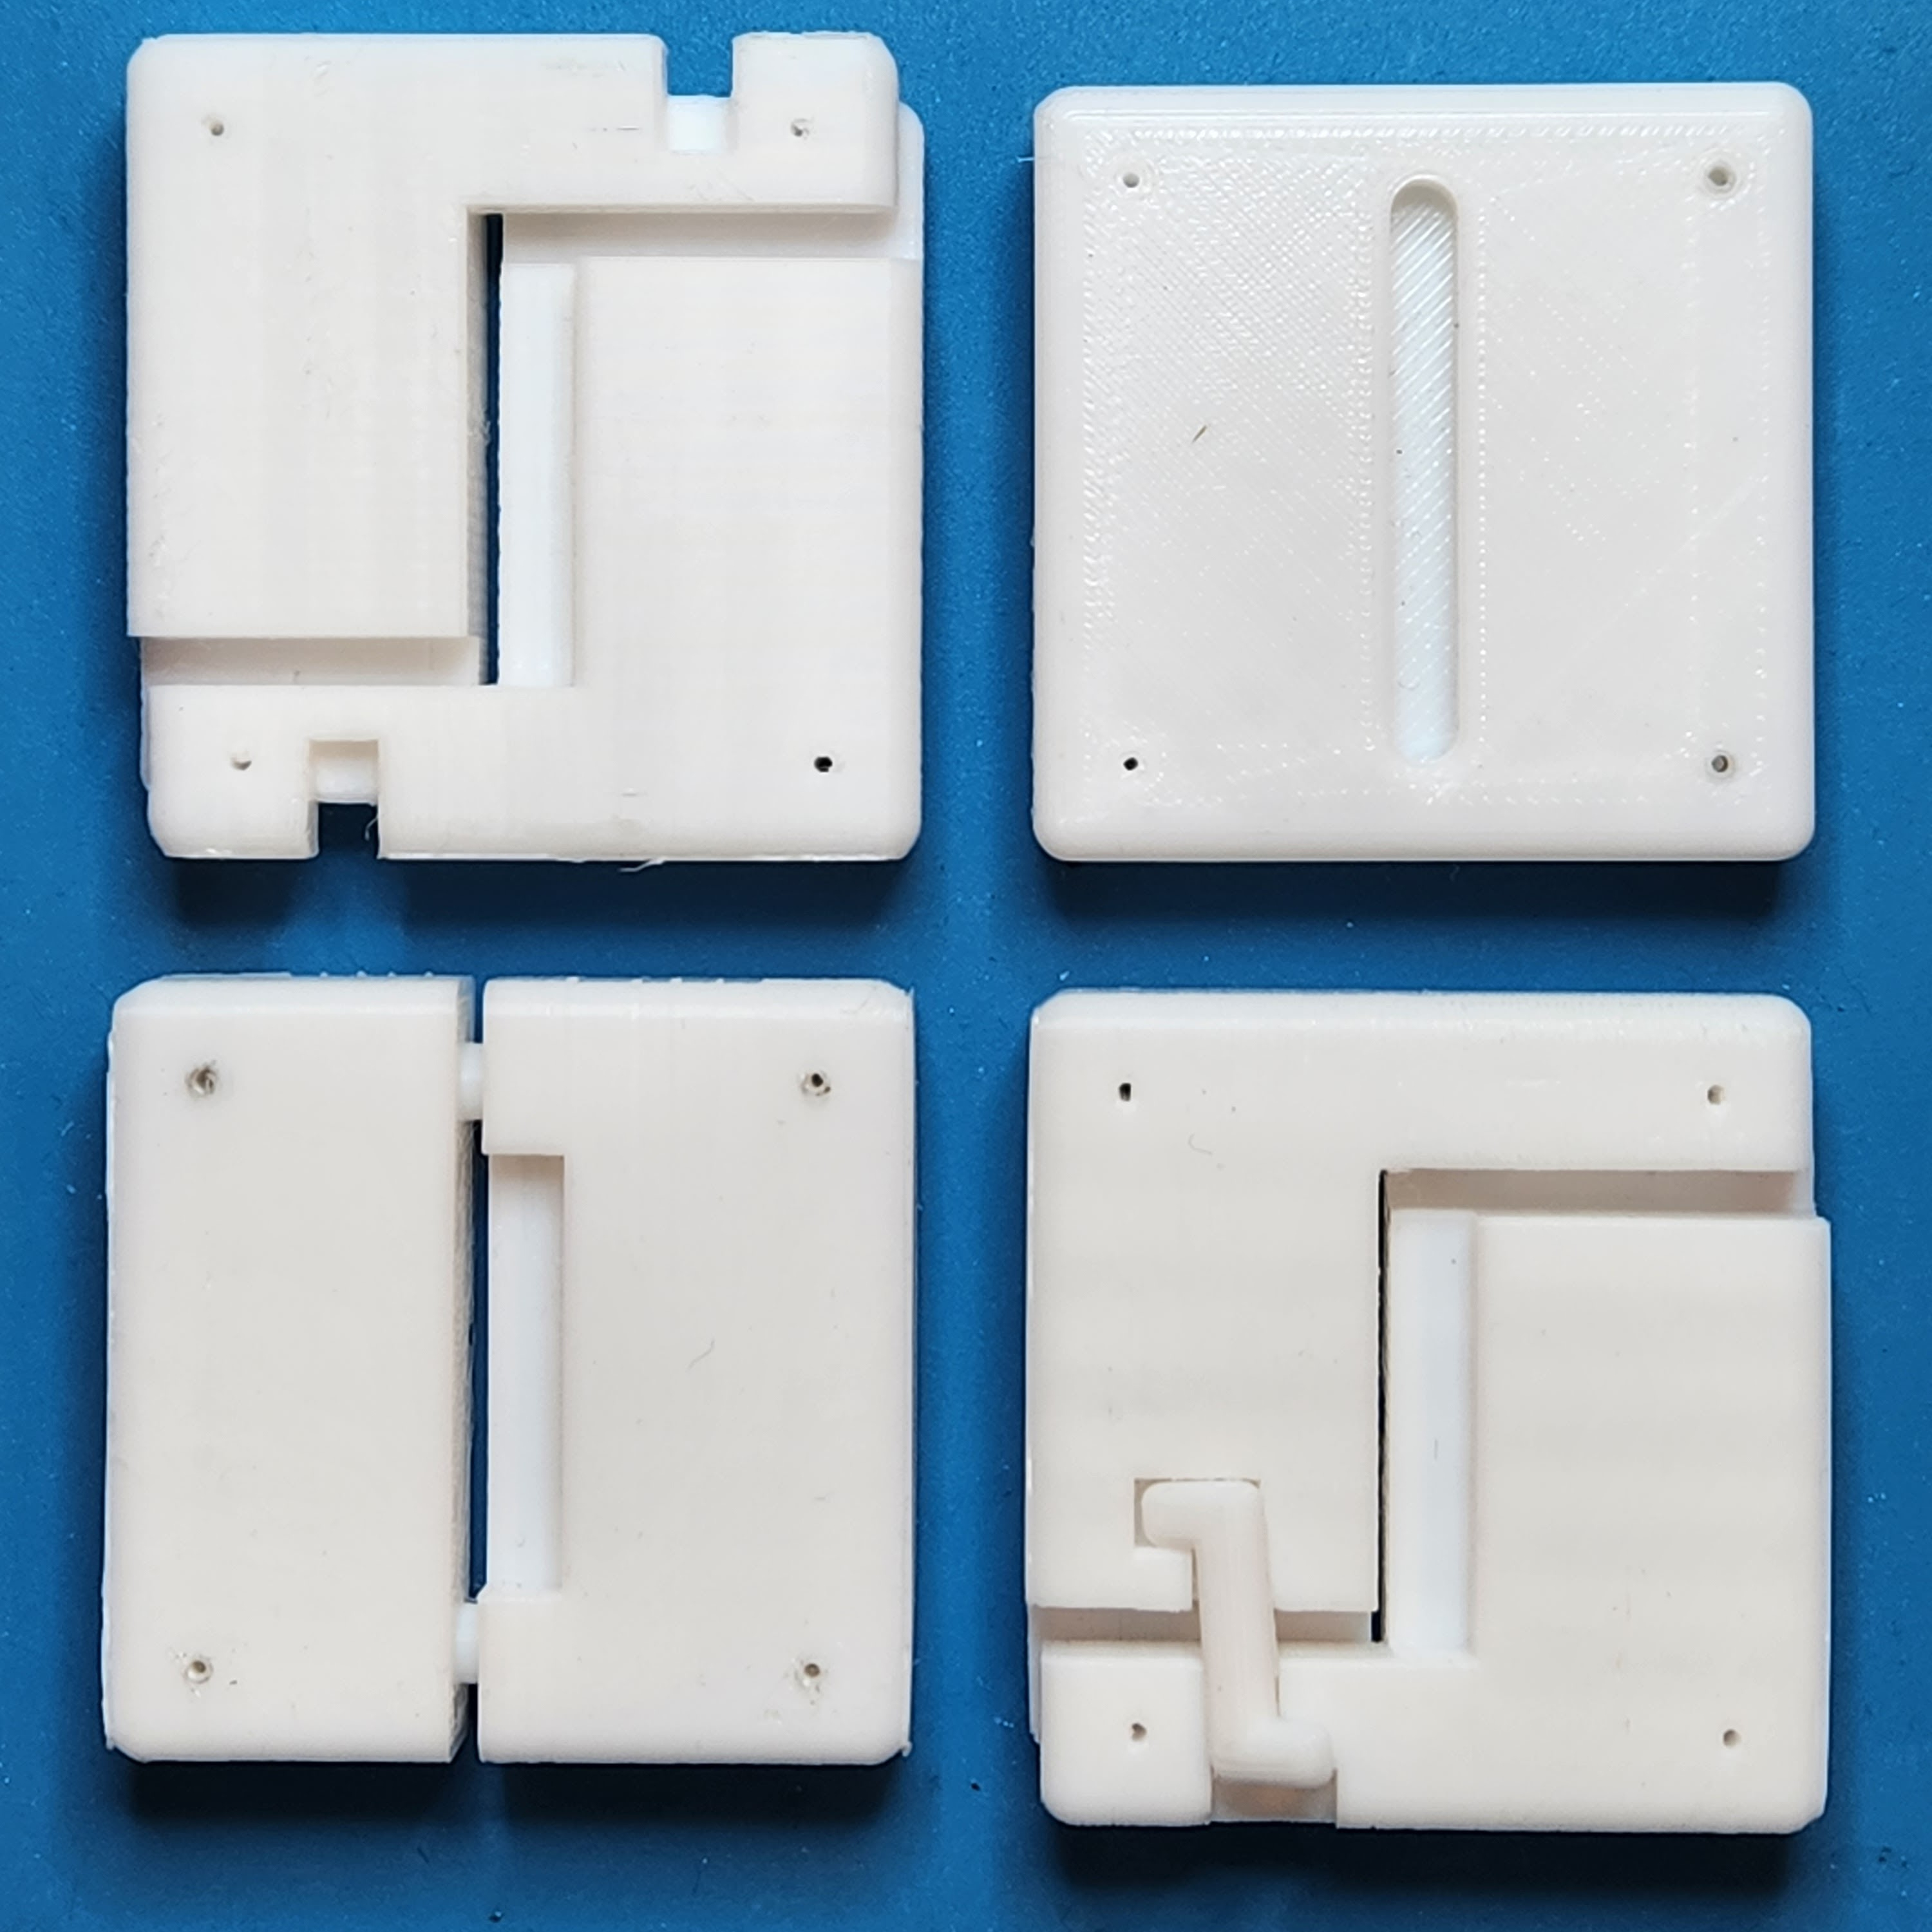
\includegraphics[width=0.6\textwidth]{Detector_description/Holder-designs.jpeg}
    \caption{3D printed cases tested to reduce risk of teflon tearing.}
    \label{fig:3d_previous_desings}
\end{figure}
